% =================================================================
% 2026 Dl4Sci Workshop poster  --  40 x 30 in, landscape
% Jiaming Pan, Nicholas Kern, Dragan Huterer (U. Michigan)
% Compile:  pdflatex astroai_poster.tex   (run from this folder)
% Drop exported notebook PNGs into  figs/  -- slots fill themselves.
% =================================================================
\documentclass{article}
\usepackage[paperwidth=101.6cm,paperheight=76.2cm,margin=1.2cm]{geometry}
\usepackage[T1]{fontenc}
\usepackage{helvet}\renewcommand{\familydefault}{\sfdefault}
\usepackage{amsmath,amssymb,bm}
\usepackage{graphicx}
\usepackage{enumitem}
\usepackage{tikz}
\usetikzlibrary{calc}
\usepackage[most]{tcolorbox}
\usepackage{qrcode}
\pagestyle{empty}
\setlength{\parindent}{0pt}

% ---- Palette (matches the roadmap figure) -----------------------
\definecolor{ink}{HTML}{1B2A4A}
\definecolor{subgray}{HTML}{5A6678}
\definecolor{paramBlue}{HTML}{2E5EAA}
\definecolor{diffPurple}{HTML}{6B4FA0}
\definecolor{fieldTeal}{HTML}{0E7C72}
\definecolor{vggOrange}{HTML}{C25E12}
\definecolor{loopRed}{HTML}{B0303C}
\definecolor{paleBg}{HTML}{F4F6FA}

% ---- Type sizes --------------------------------------------------
\newcommand{\TitleFont}{\fontsize{74}{82}\selectfont\bfseries}
\newcommand{\AuthorFont}{\fontsize{37}{45}\selectfont}
\newcommand{\BoxTitleFont}{\fontsize{36}{40}\selectfont\bfseries}
\newcommand{\BodyFont}{\fontsize{26}{32.5}\selectfont}
\newcommand{\SmallFont}{\fontsize{20.5}{26}\selectfont}
\newcommand{\TinyPosterFont}{\fontsize{18}{22}\selectfont}

% ---- Section box style -------------------------------------------
\tcbset{
  secbox/.style 2 args={
    enhanced, breakable=false,
    colback=white, colframe=#1,
    boxrule=1.8pt, arc=6mm,
    left=7mm, right=7mm, top=4mm, bottom=4.5mm,
    title={\BoxTitleFont #2},
    coltitle=white, colbacktitle=#1,
    toptitle=3mm, bottomtitle=3mm, lefttitle=8mm,
    drop fuzzy shadow=black!35,
    before skip=0mm, after skip=4.8mm
  }
}

% ---- Figure slot: shows the PNG if present, else instructions ----
% \figslot{<width>}{<height if placeholder>}{<file>}{<where to export it>}
\newcommand{\figslot}[4]{%
  \IfFileExists{figs/#3}{%
    {\centering\includegraphics[width=#1,height=#2,keepaspectratio]{figs/#3}\par}%
  }{%
    \begin{tikzpicture}
      \draw[dashed, line width=2pt, subgray, rounded corners=5mm, fill=paleBg]
        (0,0) rectangle (#1,#2);
      \node[align=center, text=subgray, text width={\dimexpr#1-4cm\relax}] at (0.5*#1,0.5*#2)
        {\SmallFont\bfseries missing figure:\ {\ttfamily\detokenize{figs/#3}}\\[3mm]\SmallFont #4};
    \end{tikzpicture}%
  }%
}

\newcommand{\hl}[2]{{\color{#1}\bfseries #2}}

\begin{document}\BodyFont\color{ink}

% ================== HEADER BAND ===================================
\begin{tikzpicture}
  \node[anchor=north west, fill=ink, rounded corners=8mm,
        minimum width=99.1cm, minimum height=12.0cm] (hdr) at (0,0) {};
  \node[anchor=west, text=white, text width=65.2cm, align=left]
    at ($(hdr.west)+(1.8cm,0.9cm)$)
    {\TitleFont Understanding the Transition from Memorization\\[2mm]
     \TitleFont\color{white!75!ink} to Generalization in Diffusion Models for Cosmology};
  \node[anchor=west, text=white!88!ink, text width=65.2cm, align=left]
    at ($(hdr.south west)+(1.8cm,1.55cm)$)
    {\AuthorFont Nicholas Kern\,$^{1}$\quad Jiaming Pan\,$^{1}$\quad Dragan Huterer\,$^{1}$
     \quad{\SmallFont $^{1}$Department of Physics, University of Michigan
     \;\;\textbullet\;\; nkern@umich.edu \;\;\textbullet\;\; 2026 DL4Sci School, LBNL}};
  \node[anchor=east, fill=white, rounded corners=4mm, inner sep=4mm,
        minimum width=18.8cm, minimum height=5.9cm]
    (litp) at ($(hdr.east)+(-12.0cm,0cm)$)
    {
\includegraphics[width=17.4cm,height=5.0cm,keepaspectratio]{figs/litp_logo.pdf}};
  \node[anchor=east, fill=white, rounded corners=4mm, inner sep=5mm]
    (qr) at ($(hdr.east)+(-1.4cm,0)$)
    {\qrcode[height=8.4cm]{https://github.com/JiamingPan/diffusion-models-simulation-data}};
\end{tikzpicture}

% Suppress the \baselineskip glue TeX would insert between the header box and
% the column row; set the gap explicitly instead (see \vspace below).
\nointerlineskip
\vspace{6mm}

% ================== THREE COLUMNS =================================
\newlength{\colw}\setlength{\colw}{31.7cm}
\begin{minipage}[t]{\colw}\vspace{0pt}
% ----------------------------------------------------------- COL 1

\begin{tcolorbox}[secbox={paramBlue}{The question}]
\SmallFont
\begin{minipage}[t]{14.6cm}
\vspace{0pt}
For inference, a trained diffusion model $s_\theta(x)$ becomes a prior over cosmological fields $x$.
If the model has memorized its training data (black points), its score (pink) will
not accurately reflect the true prior score, pushing inference to local clumps in
data space. When confronted with observational data (blue), the inferred posterior
distribution $p(x|y)$ will therefore be biased and overly confident.

\begin{enumerate}[leftmargin=9mm, itemsep=1.8mm, label=\textcolor{paramBlue}{\textbf{\arabic*.}}]
\item \hl{loopRed}{Novelty:} when do generated samples memorize training samples w.r.t. $N_{\rm train}$?
\item \hl{diffPurple}{Conditioning:} can we recover accurate posteriors on cosmological parameters, $\theta$?
\item \hl{fieldTeal}{Fidelity:} do samples retain accurate statistical properties (1 \& 2-pt functions)?
\end{enumerate}
\end{minipage}\hfill
\begin{minipage}[t]{16.0cm}
\vspace{3mm}
\centering
\figslot{16.0cm}{15cm}{inference_manifold_implication.pdf}
  {conceptual manifold schematic: learned prior, data constraint, posterior}
\end{minipage}
\end{tcolorbox}

\begin{tcolorbox}[secbox={diffPurple}{Data \& models}]
\SmallFont
\begin{itemize}[leftmargin=11mm, itemsep=2.2mm, label=\textcolor{diffPurple}{$\blacktriangleright$}]
\item \textbf{CAMELS Multifield Dataset} (IllustrisTNG; Villaescusa-Navarro
      et al.\ 2021): 1000 simulations $\to$ 128 slices each $\to$
      128k HI (neutral hydrogen) maps of size $128\times128$.
\item Six cosmological parameters:
      $\bm{\theta}=(\Omega_m,\sigma_8,A_{\mathrm{SN1}},A_{\mathrm{AGN1}},
      A_{\mathrm{SN2}},A_{\mathrm{AGN2}})$.
\item \textbf{Diffusion objective.} We corrupt a real map with noise and
      train a UNet to predict the velocity target at every noise level,
      with the cosmology $\bm{\theta}$ as conditioning.

\vspace{-1mm}
\begingroup
\fontsize{30}{36}\selectfont
\[
\begin{aligned}
x_t &= \sqrt{\bar{\alpha}_t}\,x_0+\sqrt{1-\bar{\alpha}_t}\,\epsilon,
\qquad \epsilon\sim\mathcal{N}(0,I),\\[1mm]
\mathcal{L}_{\rm diff}
&=\mathbb{E}_{x_0,\epsilon,t}\left\|
s_{\theta}(x_t,t,\bm{\theta})-\epsilon\right\|_2^2 .
\end{aligned}
\]
\endgroup
%{\TinyPosterFont\color{subgray}
%Here we use \texttt{v\_prediction}:
%$\mathrm{target}=v_t=\sqrt{\bar{\alpha}_t}\epsilon-\sqrt{1-\bar{\alpha}_t}x_0$.
%Ho et al. 2020 (DDPM).}
\item \textbf{Sampling}: 50-step DPM-Solver, $8\times$ faster than the
      500-step DDPM baseline.
\item \textbf{Training-set sweep}: Train 3 models of increasing depth (3,4,5 layer UNet), each with 6 different training set sizes: $N_{\rm train}=2^{6} \to 2^{15}$.
\end{itemize}
\end{tcolorbox}

\begin{tcolorbox}[secbox={fieldTeal}{Detecting memorization}]
\SmallFont
After training, we generate 100 novel 2D HI maps $x_j$, compare them to every
map in the model's training set $y_i$, and keep the closest match:
\begingroup
\fontsize{35}{43}\selectfont
\[
s_j = \max_i\, \mathrm{sim}(x_j,\, y_i)
\]
\endgroup
A high $s_j$ means $x_j$ is nearly a copy of one of its training map. Separately, we train a PCA encoder to map 2D images into a vector space for classification.
Here, $\mathrm{sim}$ is {\bfseries cosine similarity} (larger = more alike) measured in either pixel or PCA latent space.
For a fixed model size, the generated samples will transition from memorization to generalization at some $N_{\rm train}$ threshold.

\vspace{2mm}
\figslot{30.0cm}{14.0cm}{nf_generalize_fig2_u64_generated_vs_pixel_nn.png}
  {generated / nearest-train visual}
\end{tcolorbox}

\end{minipage}\hfill
\begin{minipage}[t]{\colw}\vspace{0pt}
% ----------------------------------------------------------- COL 2

\begin{tcolorbox}[secbox={loopRed}{Inference: do we get the correct cosmology $\theta$?}]
We ask a conditional diffusion model to generate a sample with a given cosmology $\theta_{\rm ask}$.
We pass those 2D samples to a classifier (VGG16) with an MLP head $\rightarrow\theta_{\rm rec}$, trained on our full 128k dataset.
Thus, we are able to compare the actual cosmology generated by the diffusion models $\theta_{\rm rec}$ when conditioned on an input cosmology $\theta_{\rm ask}$, which we probe as a function of training set size and model capacity.

\vspace{4mm}
\begin{center}
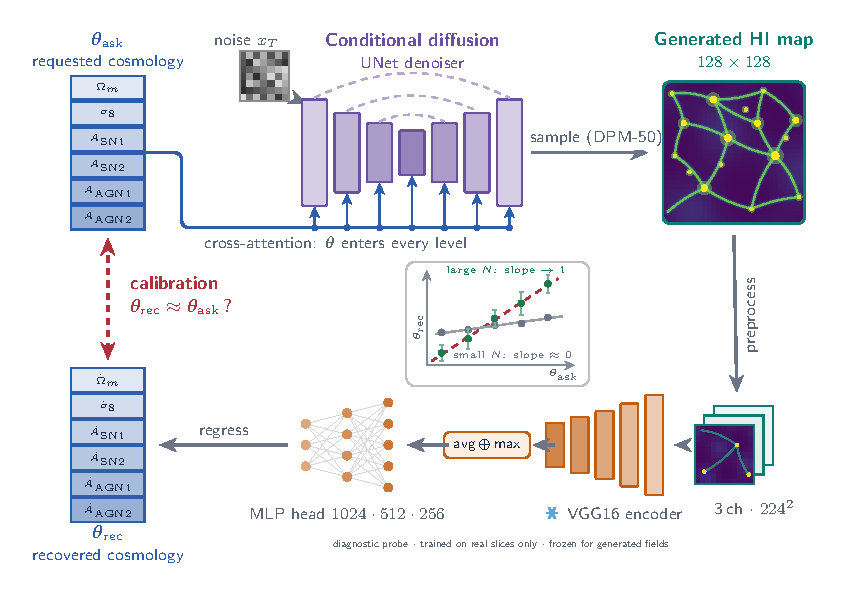
\includegraphics[width=28.2cm]{figs/calibration_roadmap_v2.pdf}
\end{center}

\end{tcolorbox}

\begin{tcolorbox}[secbox={diffPurple}{Memorization $\to$ generalization transition}]
\figslot{26.0cm}{12.4cm}{nf_generalize_fig2_poster_pca_generalization_q95_serif_clean.png}
  {quickcheck notebook $\to$ PCA generalization curves with q95 threshold}

\vspace{1mm}
For each case we generate 1000 samples: the generalization score is the fraction of generated maps that are
\emph{not} close to any training map,
\begin{center}
\vspace{1mm}
\scalebox{1.7}{$\mathrm{G} = \Pr[\, s_j < \tau \,]$\,,}
\vspace{1mm}
\end{center}
based on the cosine similarity score $s_j$, with $\tau$ (the ``memorization gap'') set by the 95th percentile of train-vs-train closest-match similarity.
\begin{itemize}[leftmargin=11mm, itemsep=2mm, label=\textcolor{diffPurple}{$\blacktriangleright$}]
\item $\mathrm{G} \approx 0$: generated samples = training samples (\hl{loopRed}{memorization}).
\item $\mathrm{G} \approx 1$: generated samples are unique to training samples.
\item The transition happens at larger $N_{\rm train}$ for larger models (is this regime predictable and universal?) {\color{subgray}(Zhang et al.\ 2024; Kadkhodaie et al.\ 2024; Yoon et
      al.\ 2023)}. Currently exploring DiTs and other cosmo datasets.
\end{itemize}
\end{tcolorbox}

\end{minipage}\hfill
\begin{minipage}[t]{\colw}\vspace{0pt}
% ----------------------------------------------------------- COL 3

\begin{tcolorbox}[secbox={vggOrange}{Calibration results}]
\begin{center}
\figslot{29.8cm}{20.8cm}{bias_probe_omega_m_best_vgg_poster.png}
  {VGG notebook $\to$ recovered vs requested $\Omega_m$ bias probe}
\end{center}

\vspace{1mm}
\SmallFont
\hl{vggOrange}{Main result:} we generate 1000 $\Omega_m$-conditional samples from two models and predict the actual $\Omega_m$ in the maps: the errorbars show 16--84\% scatter at fixed $\bm{\theta}_{\rm ask}$.
In the generalization regime (blue), the recovered $\Omega_m$ is within the true $\Omega_m$ 95\% of the time.
In the memorization regime (orange), the recovered parameters are more biased and overconfident.
The VGG+MLP encoder has $R^2=0.91$ on real held-out $\Omega_m$, so the difference is a true reflection of the diffusion model.
\end{tcolorbox}

\begin{tcolorbox}[secbox={fieldTeal}{Statistical fidelity}]
\begin{center}
\figslot{30.0cm}{14.0cm}{learning_process_pk_parallel_poster.png}
  {epoch snapshot notebook $\to$ generated and real $P(k)$ across training}
\end{center}
\vspace{1mm}
\SmallFont
Here we show that our diffusion models are indeed retaining accurate statistical information in the maps (via the 2-pt function aka power spectrum).
During training, we show the first learns large-scale features and fills-in small-scale features later in training.
\end{tcolorbox}

\begin{tcolorbox}[secbox={loopRed}{Takeaways}]
\SmallFont
\begin{enumerate}[leftmargin=12mm, itemsep=2mm, label=\textcolor{loopRed}{\textbf{\arabic*.}}]
\item \textbf{The generalization transition appears in cosmological data.} The known
      memorization-to-generalization transition also occurs in CAMELS cosmological maps.
\item \textbf{It biases inference.} Small training sets yield models that memorize: inference looks precise but is biased toward the training
      values. Past the transition, recovered cosmology $\bm{\theta}$ has better calibrated posteriors.
\item \textbf{Heuristic for practitioners.} Larger models generalize at bigger training set sizes: can we predict this transition across model \& dataset types?
\end{enumerate}
\end{tcolorbox}

\end{minipage}

\end{document}
